\section{Construcció de l'Antena}

La construcció de l'antena dipol considerada consta de dues parts: el desenvolupament del balun i la construcció del cap de l'antena.

Cal mencionar que per a realitzar la construcció de l'antena, el parametre més important considerat a estat que fos el més "low cost" possible sense comprometre la funcionalitat. Així doncs els materials utilitzats han estat:

\begin{itemize}
\item Filferro de 1.5 mm de diàmetre
\item Cable coaxial RG-95 de 75 ohms 
\item Regleta 
\item Tupper
\item Termocola
\end{itemize}

\textbf{Balun}

El balun consisteix en fer l'adaptació entre la antena y la línea de transmisió. En el nostre cas volem que l'antnea estigui adaptada per una freqüència de disseny de 121 MHz. Per realitzar-lo s'ha seguit el següent model: %(Insertar foto libro del balun realizado) 

\textbf{Cap de l'antena}

Per a la construcció del cap de l'antena s'ha utilitzat filferro de 1.5 mm de diàmetre així com una regleta per conectar els dos braços al camble d'alimentació.

A més, per tal de protegir les conexions (veure figura \ref{Conexions}), aquestes s'han dut a terme dins d'un tupper i s'han aïllat posteriorment amb termocola. A més, per temes de seguretat, a les puntes del filferro s'ha posat termocola. %\ref{capAntena} 

\begin{figure}[H]
\centering
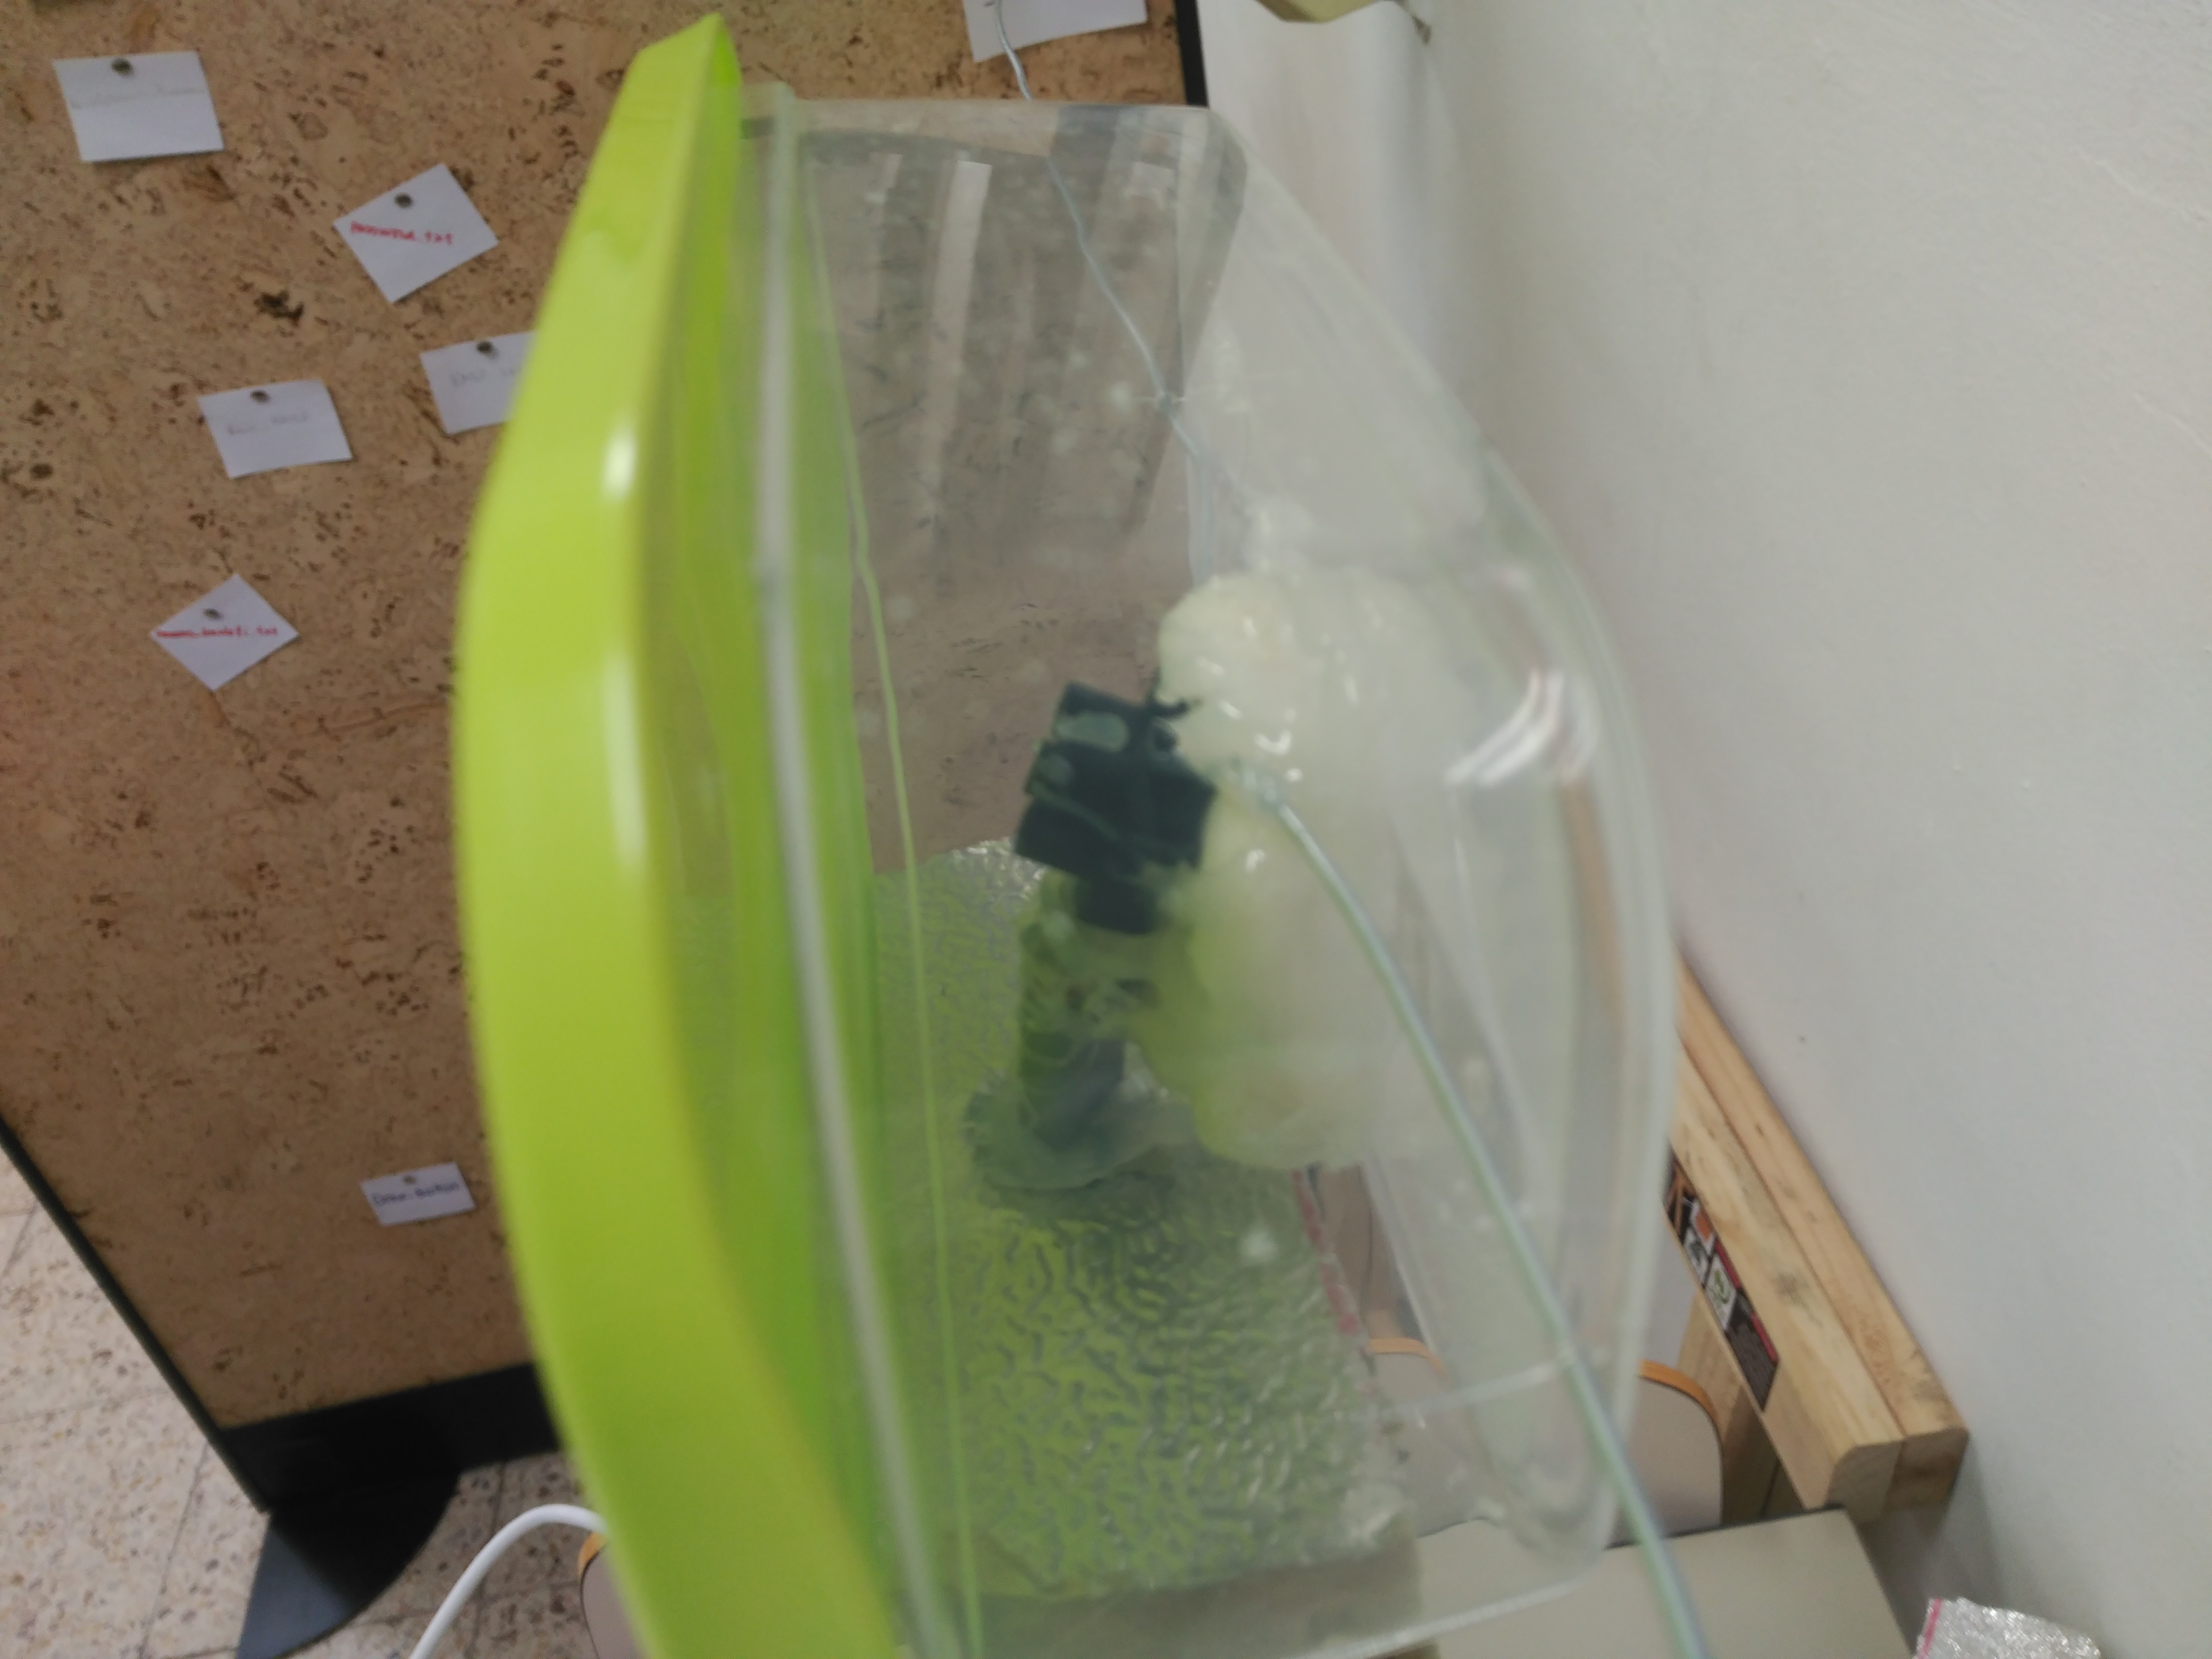
\includegraphics[width=0.5\textwidth]{./images/Conexions}
\caption{Conexions realitzades}
\label{Conexions}
\end{figure}

%((FALTA FOTO DE ANTENA DONDE SE VEAN LAS CONEXIONES))


\textbf{Antena Construida}

Finalment l'antena construida es la mostrada a la figura \ref{AntenaFinal}.

\begin{figure}[H]
\centering
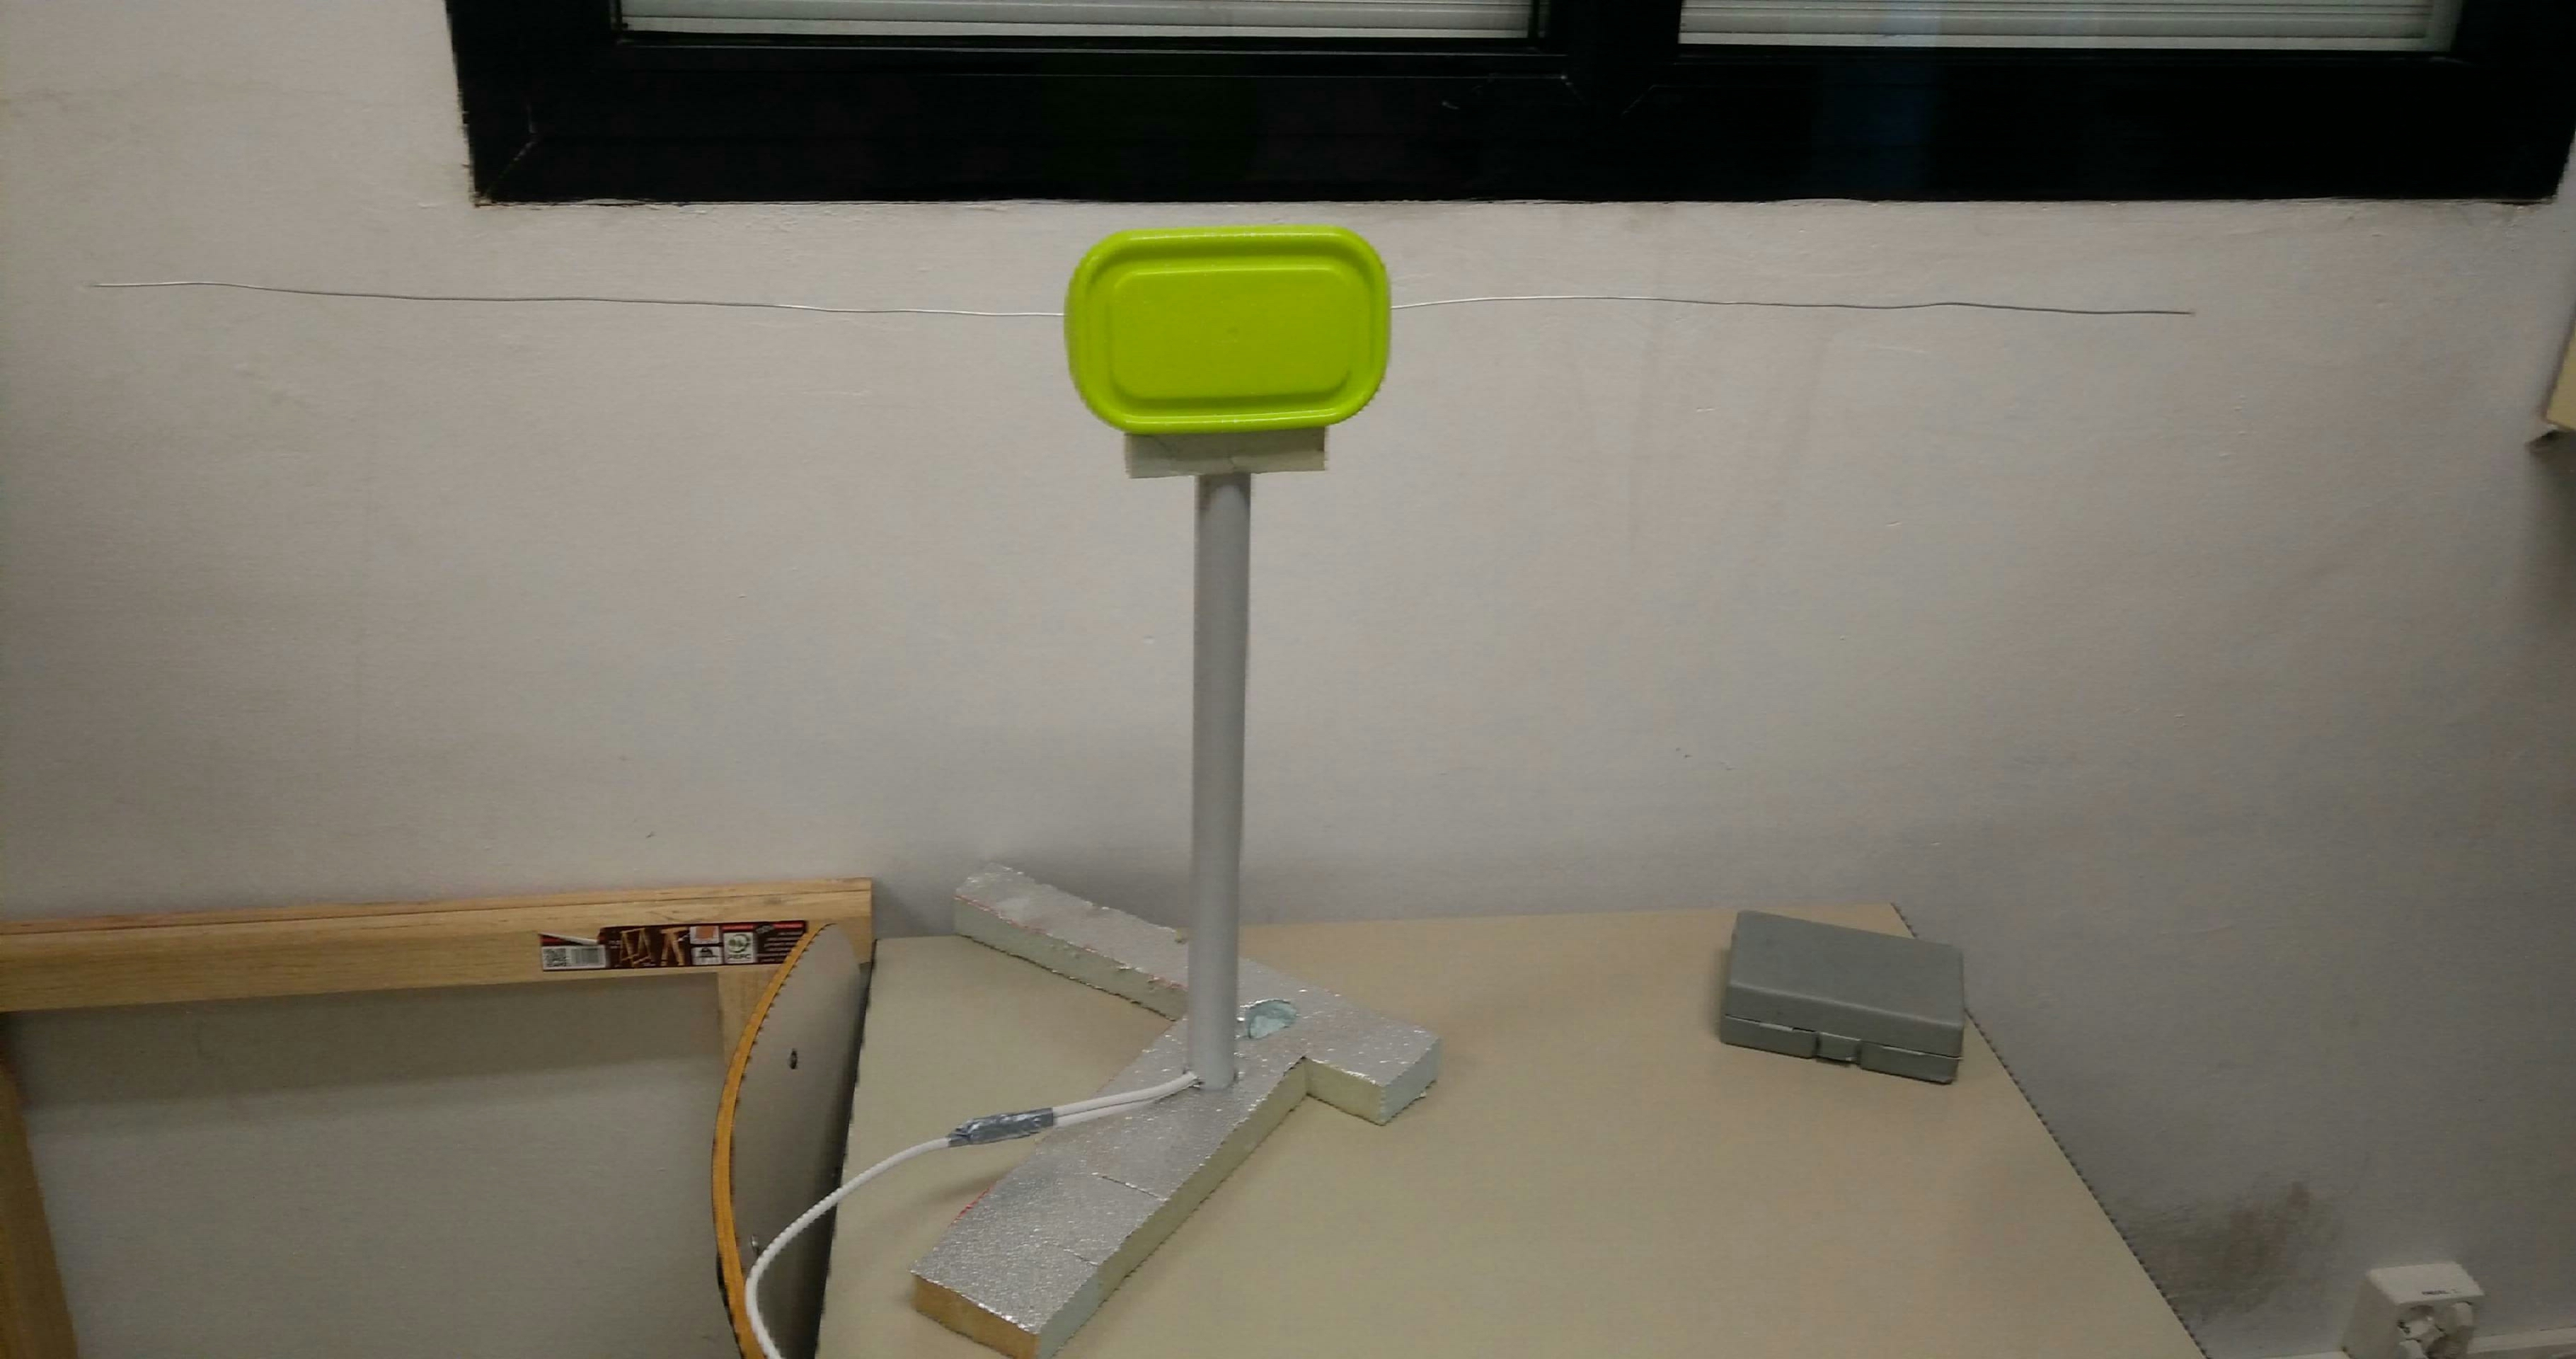
\includegraphics[width=0.8\textwidth]{./images/Antena_final}
\caption{Antena dipol construida}
\label{AntenaFinal}
\end{figure}